\documentclass[12pt]{article}

\usepackage{amsmath, amssymb, amsthm, graphicx, fancyhdr, textcomp, enumerate, diagbox, tcolorbox, esvect, tikz, adjustbox}


\graphicspath{{./images/}}


\usepackage{halloweenmath, tikzsymbols}

\newcommand{\R}{\mathbb{R}}
\newcommand{\Z}{\mathbb{Z}}
\newcommand{\C}{\mathbb{C}}
\newcommand{\N}{\mathbb{N}}
\newcommand{\Q}{\mathbb{Q}}
\newcommand{\Arg}{\mbox{Arg}}
\newcommand{\Log}{\mbox{Log}}


%geometry/topology
\newcommand{\bndry}{\partial}


\newcommand{\infsum}{\sum_{n = 1}^{\infty}}
\newcommand{\pf}{\fbox{proof}}
\newcommand{\cor}{\fbox{corollary}}

\theoremstyle{definition}

\newtheorem*{definition}{Definition}
\newtheorem{lemma}{Lemma}
\newtheorem{theorem}{Theorem}
\newtheorem{corollary}{Corollary}
\newtheorem{proposition}{Proposition}
\newtheorem{remark}{Remark}
\newtheorem{conjecture}{Conjecture}
\newtheorem{example}{Example}

\newcommand{\inv}[1]{#1^{-1}}

\title{Modern Geometry}
\author{August}

\begin{document}

\maketitle

\section{Problem 3.29}

\begin{proposition}

It is impossible for there to exist a 3-cycle subgraph of a flip graph.
\end{proposition}

\begin{proof}
Suppose we did have one. Chose any direction on the cycle, and number the edges of the graph $1$, $2$, $3$. Let $v_1$ and $v_2$ be the vertices that are the endpoints of the diagonalization that is fliped in $1$. In order for the cycle to be a cycle, we must eventually return to the original triangulation, in which case $v_1$ and $v_2$ must be re-connected by a diagonal by the remaining flips corresponding to the graph edges $2$ and $3$. Another observation is helpful: notice that the line segment between $v_1$ and $v_2$ is now blocked by the newly formed diagonal in $T_1$. As a result, it is also necessary to flip $e$ at some point. \\

There are two cases: either $2$ flips $e$ or it doesn't. Suppose first that it flips $e$ back to $T_1$. In this case, we have travelled back to the original node, and we do not have a cycle. Hence $2$ cannot flip $e$ back. Having concluded that $2$ must flip an edge other than $e$, let that edge be $f$. Let $w_1$ and $w_2$ be the original end-points of $f$ in $T_2$, so that they are not connected by an edge in $T_3$. 

We now have two pairs of vertices which are no longer connected by a diagonal, but which were connected by a diagonal in $T_1$. Notice also that each flip draws a diagonal between exactly two edges. One flip is not sufficient to re-connect $v_1$ with $v_2$, as well as $w_1$ with $w_2$. Hence we do not have a cycle: a contradiction.


\end{proof}

\section{3.24}


These triangulations are connected by no more than sixteen flips, because they are connected by six flips! See:

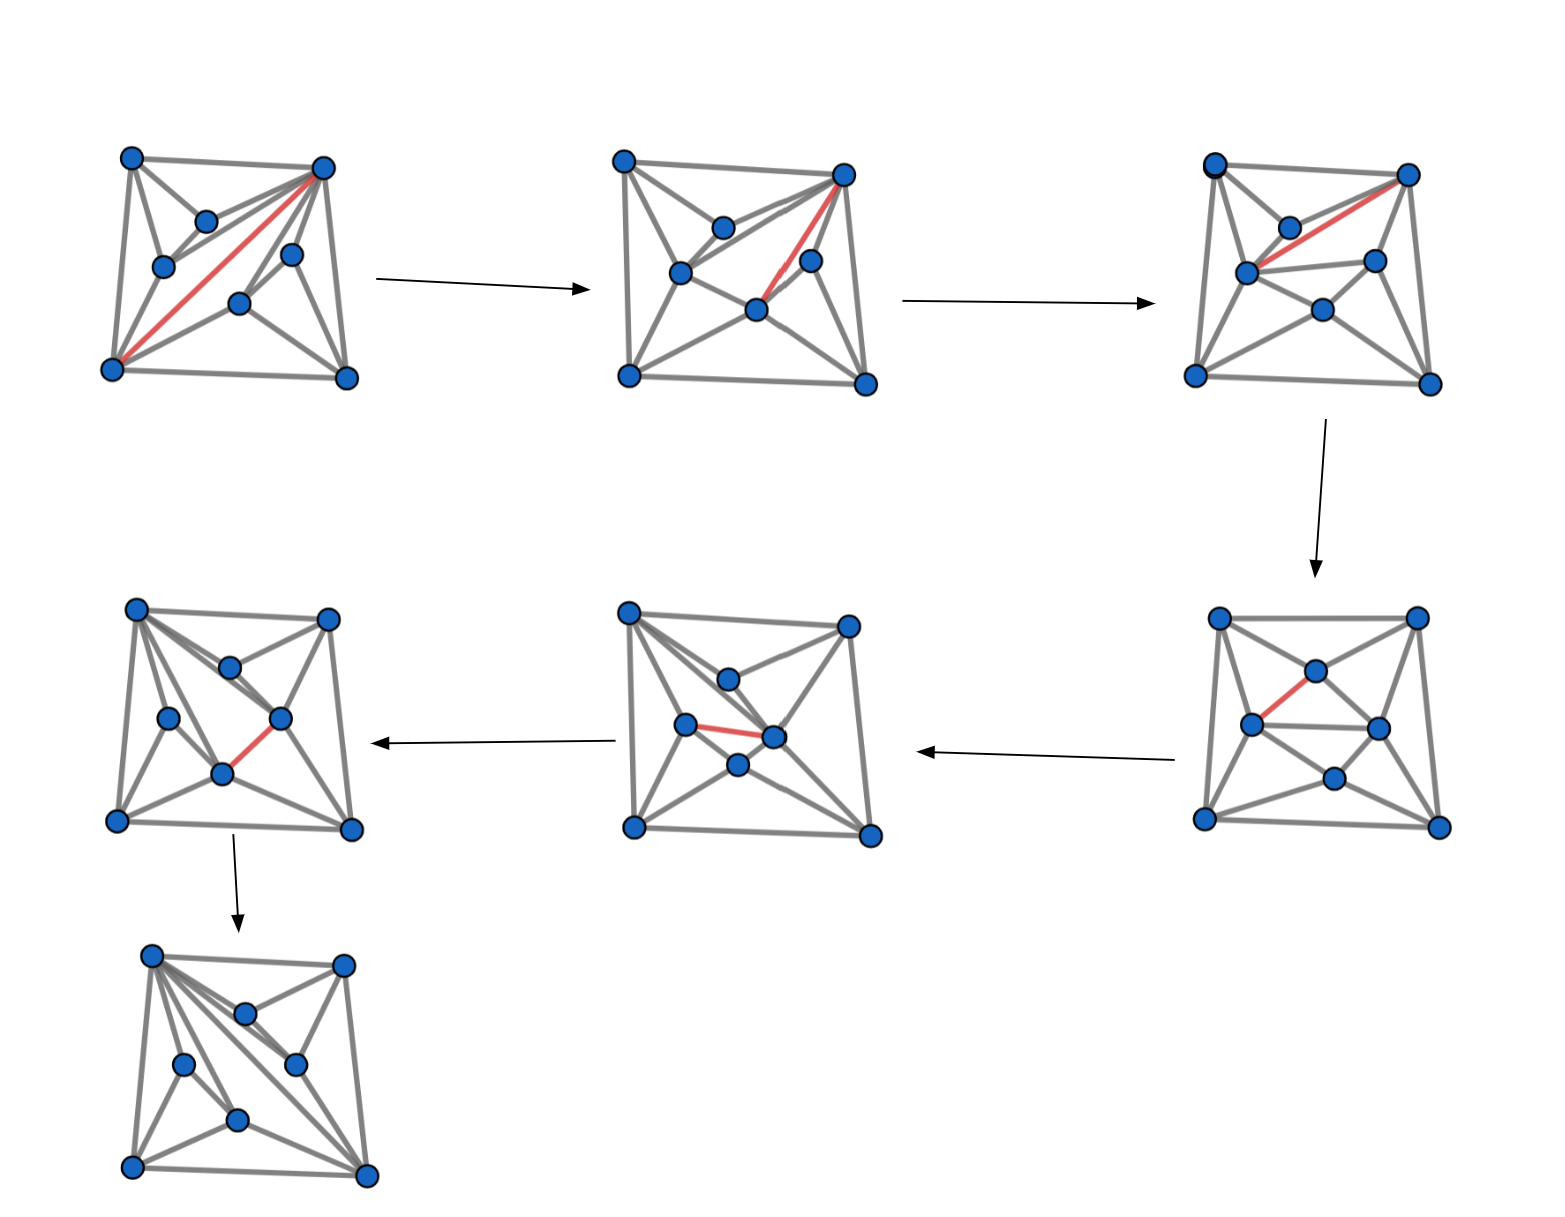
\includegraphics[scale=0.75]{flips.png} 


\section{3.52}


\begin{proposition}
Suppose that two triangles $ABC$ and $ADC$ belonging to a triangulation $T$ share the edge $AC$. Then $B$ and $D$ lie on opposite sides of the line $AC$. 
\end{proposition}

\begin{proof}
For suppose that they were on the same side of $AC$. Then there are two cases: either $B$ is inside $ACD$ or itsn't. If it is inside, then the triangle $ACD$ is split by the segment $BD$, in which case $ACD$ is not a triangle of the triangulation. \\

Moreover, if we suppose that $B$ is outside, then the edges $BA$ or $CB$ (depending on which side of the line connecting the point $D$ and the perpendicular bisector of $AC$ lie on) must cross one of the edges of the triangle $ACD$, hence it is not a diagonal, and hence $ABD$ does not belong to a triangulation.

Q.E.D.
\end{proof}

\begin{proposition}

Suppose that the triangle $ABC$ and $ADC$ share the edge $AC$, such that $B$ and $C$ lie on opposite sides of the line $AC$, and where $ABCD$ is a convex quadrilateral. Then $D$ is exterior to the circumcircle of the triangle $ABC$ if and only if $B$ is exterior to the circumcircle of the triangle $ADC$. 

\end{proposition}


\begin{proof}

First suppose tha
First suppose that $D$ is exterior to the circumcircle of the triangle 
Draw the line segment $BD$. Then since $ABCD$ is a convex quadrilateral (a bit of hand-waviness here), the line segment $BD$ intersects the line segment $AC$ at a point, call it $O$. Since the angles $\angle ADB = \delta$ and $\angle ACB = \gamma$ have a common base, since $D$ is exterior to $ABC$, and since $C$ lies on the circle $ABC$, it follows by the correct version of what the textbook calls Thales's theorem that $ \gamma > \delta $. Now let $ \kappa = \angle AOD$. Since $BOC$ is a vertical angle to $\angle AOD$, it follows that they are both equal to $\kappa$. Now let $\alpha = \angle CAD$, and let $\beta = \angle CBD$. Since the angles of a triangle sum to $\pi$, it follows that $\alpha = (\pi - \kappa)- \delta$, while $\beta = (\pi = \kappa) - \gamma$. But we have shown that $\gamma  > \delta$, hence $\alpha  > \beta$. To really drive down the  point we can substitute back in: $\angle DBC < \angle CAD$. Moreover, since these angles have a common base, and since $A $ lies on the circle $ACD$, it follows by "Thales'" "Theorem" that $B$ is exterior to the circle $ACD$. \\
Moreover, for the converse, notice that everything about this proof is symmetric in $B$ and $D$. So without loss of generality, we have proven both ways.\\

Q.E.D.
\end{proof}

More is true in the non-convex case. 

\begin{proposition}
Suppose that $ABC$ and $ADC$ are triangles sharing the edge $AC$, where $B$ and $D$ are on opposite sides of $AC$, and where $ABCD$ is not a convex quadrilateral. Then $B$ is outside the circumcircle of $ADC$, and $D$ is outside the circumcircle of $ABC$.
\end{proposition}

\begin{proof}
By symmetry, we need only prove that $B$ is outside the circumcircle of $ADC$. Since the quadrilateral is non-convex, and since $AC$ is a diagonal, it follows that either $A$ or $C$ is a reflex vertex. Without loss of generality, suppose that $A$ is a reflex vertex. Since $A$ is a reflex vertex, the angle $\angle ACB$ is greater than $\pi$, hence $B$ is on the opposite side of $A$ with respect to the line $BC$. Because the line $KC$ is tangent to the cirle $ACD$ at $C$, and since $A$ and $D$ are also part of the circle and on the other side than $D$, it follows that $D$ is not in the circumcircle, since $KC$ is a tangent and the circumcircle is a convex region.
\end{proof}
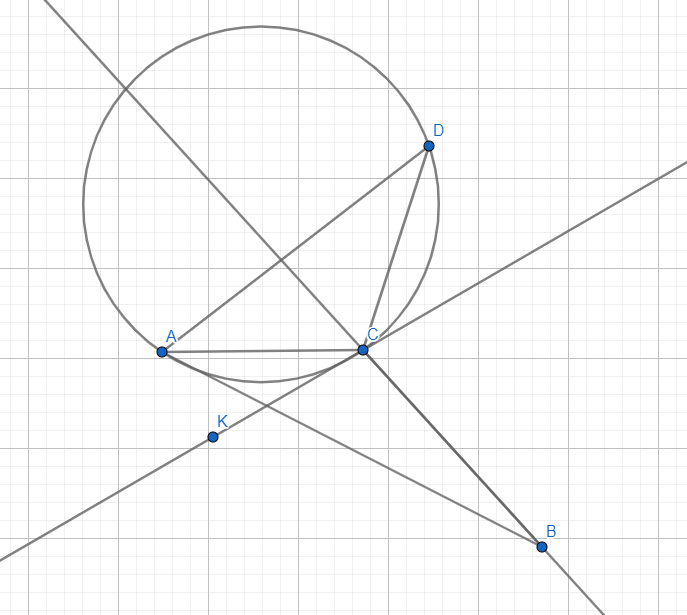
\includegraphics[scale=1]{non-convex.png} 

\section{3.61}


\begin{definition}
A compatible map between two triangulations of polygons $X$ and $Y$, $T_X$ and $T_Y$ respectively, is a bijective map from the vertices of $X$ to the vertices $Y$ which preserves triangles ($abc$ a triangle of $T_X$ implies $\phi(a)\phi(b)\phi(c)$.
\end{definition}

(note that I have un-generalized to just polygons)

\begin{lemma}
The inverse of a compatible map from convex vertices is compatible, and compatible maps preserve degrees of vertices.
\end{lemma}

\begin{proof}
It is easy to see that $\phi$ induces a map $\phi':T_X\to T_Y$, which maps triangle to triangles, and that this map is injective (since triangles are the same only if they have the same vertices). Since the number of triangles in a triangulation of a polygon is a function of the number of vertices, and since $\phi$ is a bijection from the vertices of $X$ to the vertices of $Y$ (hence they have the same number of elements), it follows that $T_X$ and $T_Y$ are both of the same size. So we have an injection from two finite sets of the same size, so $\phi'$ is a bijection, and it must have an inverse. Now notice that this inverse is induced by a function from the vertices of $Y$ to the vertices of $X$, and that this function, when composed with $\phi$, is the identity, hence this function is the inverse of $\phi$, and it maps triangles to triangles.


First, it's easy to see that $\phi:X \to Y$ respects diagonals and edges. If $ab$ is a diagonal or edge of $X$, then it is part of some triangle $abc$, which is sent to the triangle $\phi(a)\phi(b)\phi(c)$. Hence $\phi(a)\phi(b)$ is either an edge or diagonal. Now let $p$ be a point, and let $pa$ be a diagonal or edge connecting to $p$. Then $\phi(p)\phi(a)$ is also a diagonal connecting to $\phi(p)$. Moreover, each of these is distinct, so it follows that this induced map from diagonals of to $p$ to diagonals to $\phi(p)$ is injective, so $\deg p \le \deg \phi(p)$. Applying the same argument for $\phi(p)$ and using the compatible map $\inv{\phi}$, we find that $\deg p \ge \deg \phi(p)$. Hence $\deg p = \deg{\phi(p)}$.\\

This concludes the proof, and shows that degrees are invariant under compatible maps. Q.E.D.


\end{proof}



Now consider this pair of polygons: \\

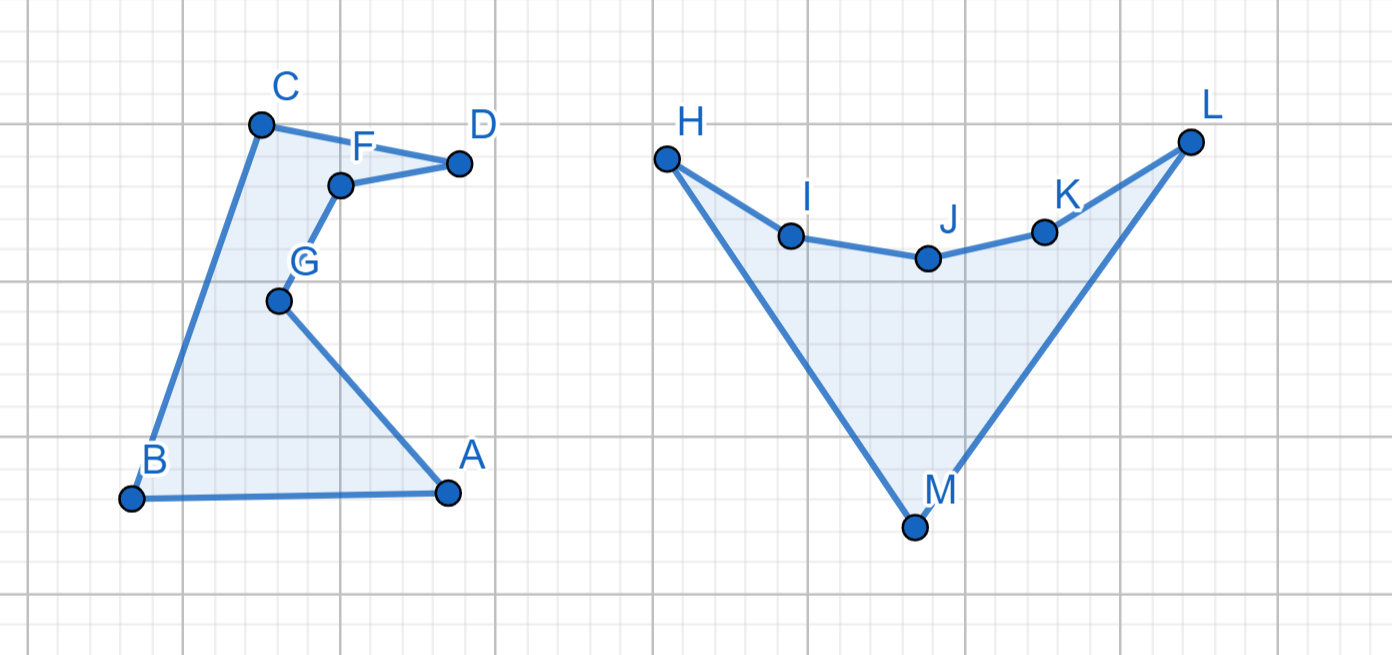
\includegraphics[scale=0.5]{counterexample.png} 

As I showed in a previous assignment, the one on the right has only one triangulation, and in that triangulation the vertex $M$ has degree $5$. Now notice that it is only possible for a vertex to have degree $5$ among six vertices if an edge connects to all the rest. In the polygon on the left, no vertex can see all the others, hence do vertex has degree $5$ in any triangulation. Since, as I have shown, compatible maps preserve degrees, it follows that these shapes are not compatible.

Q.E.D.

\section{Problem b}

\begin{proposition}
There exists a point set with four vertices which has no Pittaway triangulation.
\end{proposition}

\begin{proof}
Consider this point set (where the red points are not part of the point set.)

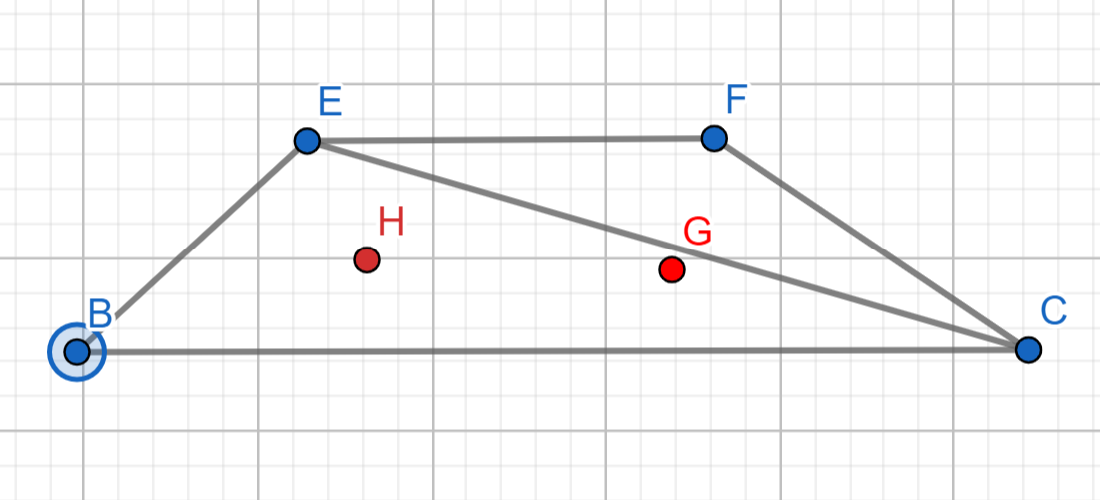
\includegraphics[scale=1]{not_pittaway.png} 

Recall that a convex quadrilateral has exactly two triangulations. Since this one is symmetric, without loss of generality suppose we have the triangulation above, where the diagonal $ EC $ is drawn. Then the point $G$ is closest to $F$, which is not a vertex of the triangle $EBC$, which contains it. A similar thing happens if the diagonal $FB$ is drawn, in which case $H$ is closest to $E$. 
\end{proof}

I think I have a rigorous that such a construction actually works. Using this proof, I think I can show how this construction can be extended to provide a point set with no pittaway triangulation for $n>3$.


\section{Problem a}

\begin{proposition}
The only two dimensional facets of an $n$-dimensional associahedron are 4-cycles and 5-cycles.
\end{proposition}

\begin{proof}
Recall that the diagonalizations with all but two diagonals of a triangulation are in one-to-one correspondence with the two dimensional facets, and the number of nodes of those facets are the number of trianguliations corresponding to this diagonalization. So for any face, the corresponding diagonalization has two cases: either the two missing diagonals are adjacent to each other or they are not. If they are not adjacent, we have two quadrilaterals, each having two triangulations. Since each of these have two triangulations, in all we have four of them, hence a 4-cycle. If the two missing diagonals are adjacent, we have ourselves a convex pentagon. Since the flip graph of the convex pentagon is the two dimensional associahedron, which is a five cycle, we have ourselves a five cycle. In either case, we have 4-cycles and 5-cycles. Hence the only two dimensional facets of an $n$-dimensional associahedron are 4-cycles and 5-cyles. 

Q.E.D.


\end{proof}

\begin{proposition}
For all $n$-dimensional associahedra, $n$ of the $n-1$ dimensional facets are $n-1$-dimensional associahedra. Moreover, every node belongs to one such facet, and is connected to a distinct other facet by an edge in the flip graph.
\end{proposition}

\begin{proof}
We proceed by induction. For the base case, consider the line. Clearly it's zero dimensional facets are points, which are zero dimensional associahedra, and they are connected by the single edge. Suppose the proposition holds for all $n-1$ dimensional associahedra. Now suppose that we have some $n$-dimensional associahedron, corresponding to the flip graph of an $n+3$ vertex convex polygon $P$. Since $P$ is a convex polygon, it follows that each of the $n+3$ vertices is an ear. Hence at least one vertex is triangled off, and each triangulation corresponds to some such ear, leaving us with a convex $n+2$-gon, whose flip graph is the $n-1$ dimensional associahedron. Since there will always be one more adjacent edge next to the one triangling off our ear, it these nodes are all connected to a distinct flip, which would make the nieghboring ear triangled off. This neighboring ear corresponds to yet another $n-1$ dimsenional associahedron. So the proposition holds in the inductions step as well. 
Q.E.D.
\end{proof}

\end{document}
